\documentclass[11pt,a4paper]{article}

\usepackage[a4paper,margin=2.35cm,headheight=14pt]{geometry}
\usepackage{fontspec}
\IfFontExistsTF{Georgia}{\setmainfont{Georgia}}{\setmainfont{Latin Modern Roman}}
\IfFontExistsTF{Helvetica}{\setsansfont{Helvetica}}{\setsansfont{Latin Modern Sans}}
\usepackage{microtype}
\usepackage{booktabs}
\usepackage{graphicx}
\usepackage{amsmath}
\usepackage{amssymb}
\usepackage{natbib}
\usepackage{xcolor}
\usepackage{hyperref}
\usepackage{fancyhdr}
\usepackage{caption}
\usepackage{float}
\usepackage{enumitem}
\usepackage{setspace}

\definecolor{ink}{HTML}{222222}
\definecolor{muted}{HTML}{555555}
\definecolor{accent}{HTML}{2166AC}
\hypersetup{
  colorlinks=true,
  linkcolor=accent,
  citecolor=accent,
  urlcolor=accent,
  pdftitle={The Economic Geography of Europe: Regional Disparities in GDP per Capita},
  pdfauthor={Reproducible empirical study}
}
\captionsetup{font=small,labelfont=bf}
\setlength{\parindent}{1.2em}
\setlength{\parskip}{0.15em}
\linespread{1.04}
\setlist[itemize]{leftmargin=1.5em,itemsep=0.15em,topsep=0.25em}
\graphicspath{{../figures/}}

\pagestyle{fancy}
\fancyhf{}
\lhead{\footnotesize\textsf{The Economic Geography of Europe}}
\rhead{\footnotesize\textsf{2023 NUTS 2 evidence}}
\cfoot{\thepage}
\renewcommand{\headrulewidth}{0.3pt}

% Generated by src/analysis.py. Do not edit by hand.
\newcommand{\NRegions}{276}
\newcommand{\NEURegions}{244}
\newcommand{\NCandidateRegions}{32}
\newcommand{\NCountries}{31}
\newcommand{\MeanGDP}{89.6}
\newcommand{\MedianGDP}{84}
\newcommand{\SDGDP}{36.7}
\newcommand{\CVGDP}{0.410}
\newcommand{\GiniGDP}{0.219}
\newcommand{\TheilGDP}{0.078}
\newcommand{\PtenGDP}{50}
\newcommand{\PninetyGDP}{131}
\newcommand{\PninetyTen}{2.62}
\newcommand{\BelowSeventyFive}{39.1}
\newcommand{\AtLeastHundred}{33.7}
\newcommand{\BetweenCountryShare}{54.2}
\newcommand{\MinRegionName}{Şanlıurfa, Diyarbakır}
\newcommand{\MinRegionCode}{TRC2}
\newcommand{\MinRegionValue}{26}
\newcommand{\MaxRegionName}{Eastern and Midland}
\newcommand{\MaxRegionCode}{IE06}
\newcommand{\MaxRegionValue}{251}
\newcommand{\QueenEdges}{590}
\newcommand{\QueenIsolates}{21}
\newcommand{\QueenComponents}{25}
\newcommand{\MoranN}{255}
\newcommand{\MoranI}{0.600}
\newcommand{\MoranP}{0.00001}
\newcommand{\MoranRawI}{0.460}
\newcommand{\MoranEUI}{0.503}
\newcommand{\MoranRookI}{0.599}
\newcommand{\LISAHH}{4}
\newcommand{\LISALL}{16}
\newcommand{\LISAHL}{1}
\newcommand{\LISALH}{0}
\newcommand{\LISAFDRTotal}{21}
\newcommand{\LISAHolmTotal}{9}
\newcommand{\NProvisional}{101}
\newcommand{\NEstimated}{1}
\newcommand{\Permutations}{99,999}


\title{\vspace{-1.2cm}\textbf{The Economic Geography of Europe:}\\[0.25em]
\Large Regional Disparities in GDP per Capita}
\author{\normalsize Reproducible empirical study}
\date{\normalsize 23 July 2026}

\begin{document}
\color{ink}
\maketitle
\thispagestyle{fancy}

\begin{abstract}
\noindent
This paper measures the magnitude and spatial organization of regional economic
disparities in Europe using Eurostat's 2023 GDP-per-capita index and NUTS 2024
level-2 boundaries. An exact one-to-one inner join produces \NRegions{} regions:
\NEURegions{} in the EU27 and \NCandidateRegions{} in four candidate countries.
Across equally weighted regions, the median index is \MedianGDP{}, the Gini
coefficient is \GiniGDP{}, and the 90-to-10 percentile ratio is
\PninetyTen{}. Spatial association is assessed on log GDP per capita using
row-standardized first-order queen contiguity. After excluding \QueenIsolates{}
regions without a contiguity neighbor, global Moran's $I$ is \MoranI{}
($p=\MoranP{}$, \Permutations{} random-label permutations). The result remains
large under raw-index, rook, EU-only, largest-component, and nearest-neighbor
specifications. Benjamini-Hochberg-adjusted local Moran statistics identify
\LISAHH{} high-high, \LISALL{} low-low, and \LISAHL{} high-low regions. These
results establish a pronounced descriptive spatial pattern, not causal
spillovers, convergence, or the effects of any particular regional policy.
\end{abstract}

\noindent\textbf{Keywords:} regional inequality; GDP per capita; NUTS 2;
spatial autocorrelation; Moran's I; Europe

\section{Introduction}

Large differences in regional productivity and income generation remain central
to European economic policy. The relevant geography is not only national:
capital regions, corporate centers, industrial belts, rural peripheries, and
border areas can differ sharply within the same country. At the same time,
neighboring regions share markets, infrastructure, institutions, and history.
Regional inequality and spatial clustering are therefore distinct empirical
questions. Dispersion measures describe how unequal regional values are, while
spatial statistics ask whether similar values are located near one another.

This paper asks: \emph{How strongly, and where, was 2023 GDP per capita
spatially clustered among neighboring NUTS 2 regions with available Eurostat
data?} It makes three contributions. First, it constructs an auditable
cross-section from two official snapshots and documents the exact coverage
created by the requested inner join. Second, it reports region-equal
distributional statistics and a complete choropleth with insets for outermost
regions. Third, it combines global and local Moran statistics with permutation
inference, explicit zero-neighbor treatment, multiple-testing adjustment, and
prespecified sensitivity checks.

The evidence is clear but deliberately descriptive. The region-equal mean is
\MeanGDP{} and the median is \MedianGDP{} relative to an EU27 benchmark of
100. The spatial result is stronger still: Moran's $I$ for log GDP per capita is
\MoranI{}, compared with a random-label expectation near zero. The pattern is
robust to alternative variable transformations, weights, and samples. Local
evidence is more selective: \LISAFDRTotal{} regions are retained after
Benjamini-Hochberg adjustment, of which \LISALL{} form low-low cores. Nothing in
this one-year design identifies why the pattern arose.

\section{Literature review}

The theoretical starting point is the possibility that economic activity
concentrates endogenously. In the core-periphery model of \citet{krugman1991},
increasing returns, transport costs, and market-size feedback can produce
agglomeration. That mechanism is a useful interpretation of clustered
production, but a cross-sectional map cannot test it. A separate growth
literature studies beta and sigma convergence. \citet{salaimartin1996}
distinguishes faster growth among initially poorer regions from declining
cross-sectional dispersion. A single 2023 observation tests neither.

European empirical work has long emphasized the spatial distribution rather
than only an average convergence coefficient. \citet{lopezbazo1999} connect
distributional dynamics and spatial association across EU regions.
\citet{legalloertur2003} use global and local spatial statistics to document
persistent high- and low-income clusters in 138 European regions over
1980--1995. \citet{ertur2006} further show that spatial dependence and spatial
regimes matter for estimated convergence processes. More recently,
\citet{iammarino2019} synthesize the heterogeneous trajectories behind
European regional inequality and caution against one-size-fits-all
interpretations. The Ninth Cohesion Report likewise describes EU-wide
convergence alongside persistent territorial challenges
\citep{ec2024cohesion}.

The present study updates the descriptive spatial cross-section without
claiming a convergence test. Global spatial association is measured with
Moran's $I$ \citep{moran1950}; local cluster cores and spatial outliers are
identified with Anselin's local indicators of spatial association
\citep{anselin1995}. Because hundreds of local hypotheses are examined, the
main map uses the adjustment proposed by \citet{benjaminihochberg1995}.

\section{Data}

\subsection{Economic and geographic sources}

The economic input is Eurostat dataset \texttt{nama\_10r\_2gdp}, ``Gross
domestic product at current market prices by NUTS 2 region''
\citep{eurostat2026gdp}. The API query filters 2023 and unit code
\path{PPS_HAB_EU27_2020}; the response records annual frequency. The index
expresses purchasing power standard per inhabitant as a percentage of the EU27
average. Its benchmark of 100 is population weighted, not the mean of NUTS 2
observations; an equally weighted regional mean need not equal 100.

The downloaded CSV has 416 unique geographic keys: 31 national values, 108
NUTS 1 values, 276 NUTS 2 values, and the EU27 aggregate. The geographic input
is the GISCO NUTS 2024 level-2 region shapefile at 1:20 million resolution in
WGS 84 (EPSG:4326) \citep{gisco2026}. NUTS 2 denotes ``basic regions for
regional policies,'' and the 2024 classification is valid from 1 January 2024
\citep{eurostat2026nuts}. The raw geometry contains 299 valid, unique level-2
features.

\subsection{Cleaning, join, and sample}

Identifiers are preserved as strings, including meaningful zeroes, and the
economic constants, numeric values, uniqueness, projection, geometry validity,
and NUTS level are asserted before joining. A one-to-one inner join of CSV
\texttt{geo} to shapefile \texttt{NUTS\_ID} yields \NRegions{} regions and no
unmatched GDP-side NUTS 2 key. The inner join itself removes every national,
NUTS 1, and EU aggregate, exactly as required.

The resulting sample is broader than the EU27: it contains all \NEURegions{}
EU NUTS 2 regions plus \NCandidateRegions{} regions in Montenegro, North
Macedonia, Serbia, and Türkiye. Twenty-three mapped regions have no selected
GDP observation: Albania (3), Bosnia and Herzegovina (3), Switzerland (7),
Iceland (1), Liechtenstein (1), Norway (7), and Kosovo (1). The estimand is
therefore the set of Eurostat NUTS 2 regions with an available value, not every
region conventionally understood as Europe.

Eurostat marks \NProvisional{} joined observations provisional and
\NEstimated{} estimated. These flags are retained. The analysis does not
transform the archived source files; byte sizes, SHA-256 hashes, URLs,
retrieval date, anti-joins, edge lists, software versions, and every derived
output accompany the paper.

\subsection{Measurement}

GDP per capita measures production located in a region, not disposable
household income or welfare. Commuting can separate workplace production from
residence, and the regional location of multinational profits can elevate
corporate centers \citep{eurostat2025regionalgdp}. Moreover, regional
purchasing-power parities do not exist; Eurostat applies national conversion
factors within each country
\citep{eurostat2026metadata}. The analysis therefore treats the index as a
harmonized production measure and does not attach welfare interpretations to
small differences.

\section{Methods}

\subsection{Distributional description}

Each NUTS 2 region receives equal weight because the selected file contains no
population field. Reported statistics include the mean, median, standard
deviation, coefficient of variation, percentile ratio, Gini coefficient, and
Theil $T$. They describe the distribution across administrative regions, not
across people. For additional geographic context, a one-way decomposition
reports the share of total log-index sum of squares located between country
means. This is descriptive variance accounting, not a causal country effect.

\subsection{Spatial weights and global association}

The prespecified outcome for spatial inference is
$x_i=\log(\text{GDP index}_i)$. Logging makes proportional gaps more symmetric
and reduces leverage from a few corporate and capital regions; the unlogged
index is retained as a sensitivity check. The primary binary graph links
regions whose generalized polygons share a boundary or point (first-order
queen contiguity). Its \QueenEdges{} undirected edges are row standardized:
\[
  w_{ij}^{R}=\frac{w_{ij}}{\sum_j w_{ij}}.
\]
The graph has \QueenIsolates{} zero-neighbor regions and \QueenComponents{}
components. Zero-neighbor regions remain in every descriptive table and map
but are not assigned an artificial neighbor. Spatial inference uses the
induced graph of the remaining \MoranN{} regions, re-centering the outcome in
that sample.

For centered values $z_i=x_i-\bar{x}$, global Moran's statistic is
\[
 I=\frac{n}{S_0}
   \frac{\sum_i\sum_j w_{ij}^{R}z_i z_j}
        {\sum_i z_i^2},
 \qquad S_0=\sum_i\sum_jw_{ij}^{R}.
\]
The null is random labeling of the observed values over the fixed graph. A
one-sided greater test uses \Permutations{} permutations and the finite
simulation correction
\[
 p=\frac{1+\#\{I^{(b)}\ge I_{\mathrm{obs}}\}}{B+1}.
\]
This evaluates positive spatial association, not sampling uncertainty in the
Eurostat estimates.

\subsection{Local association and robustness}

For each region with at least one contiguity neighbor, Anselin's local
statistic is proportional to $z_i\sum_j w_{ij}^{R}z_j$. Conditional
randomization holds the focal $z_i$ fixed and samples neighbor values without
replacement from the other regions.
Two-sided local $p$-values are centered on each region's permutation
distribution. Quadrants are defined by the signs of $z_i$ and its spatial lag:
high-high (HH), low-low (LL), high-low (HL), and low-high (LH). ``High'' and
``low'' are relative to the spatial-analysis sample center, not necessarily to
the EU benchmark of 100.

The main local result applies Benjamini-Hochberg adjustment at nominal
$q=0.05$ across all \MoranN{} tests. Holm-adjusted results provide a stricter
family-wise-error check. Global sensitivity specifications use the raw index,
a rank-normal transformation, rook contiguity, an EU27-only sample, the
largest connected component, and a symmetric 5-nearest-neighbor graph on that
component. Nearest-neighbor centroids and distances are calculated only after
projection to EPSG:3035.

\section{Results}

\subsection{Magnitude of regional disparities}

\begin{table}[H]
\centering
\caption{Region-equal descriptive statistics, 2023}
\label{tab:descriptive}
\begin{tabular}{lr}
\toprule
Statistic & Value \\
\midrule
Regions & 276 \\
Countries & 31 \\
Mean & 89.6 \\
Median & 84.0 \\
Standard deviation & 36.7 \\
Coefficient of variation & 0.410 \\
10th percentile & 50.0 \\
90th percentile & 131.0 \\
90/10 ratio & 2.620 \\
Gini coefficient & 0.219 \\
Theil T & 0.078 \\
Share below 75 & 39.1\% \\
Share at or above 100 & 33.7\% \\
Between-country share of log variance & 54.2\% \\
\bottomrule
\end{tabular}

\begin{minipage}{0.82\textwidth}
\vspace{0.4em}\footnotesize
\textit{Notes:} GDP per capita is an index with EU27 population-weighted
average equal to 100. Shares and distributional statistics weight every
region equally. The between-country entry is the share of total log-index sum
of squares accounted for by deviations of country means.
\end{minipage}
\end{table}

Table~\ref{tab:descriptive} shows substantial dispersion. The index ranges from
\MinRegionValue{} in \MinRegionName{} (\MinRegionCode{}) to
\MaxRegionValue{} in \MaxRegionName{} (\MaxRegionCode{}). The median is
\MedianGDP{}, the standard deviation is \SDGDP{}, and the coefficient of
variation is \CVGDP{}. The 90th-percentile region has \PninetyTen{} times the
index of the 10th-percentile region. The Gini coefficient is \GiniGDP{} and
Theil $T$ is \TheilGDP{}.

\BelowSeventyFive{}\% of regions fall below 75, while only
\AtLeastHundred{}\% reach or exceed the EU benchmark. These are regional
fractions, not population shares. Country means account for
\BetweenCountryShare{}\% of log-index variation, leaving a large
within-country component as well. Figure~\ref{fig:gdpmap} makes both structures
visible: lower values are common in the east and southeast, but high capital
or metropolitan regions appear within several lower-income countries, while
important internal gradients are also visible in western member states.

\begin{figure}[H]
\centering
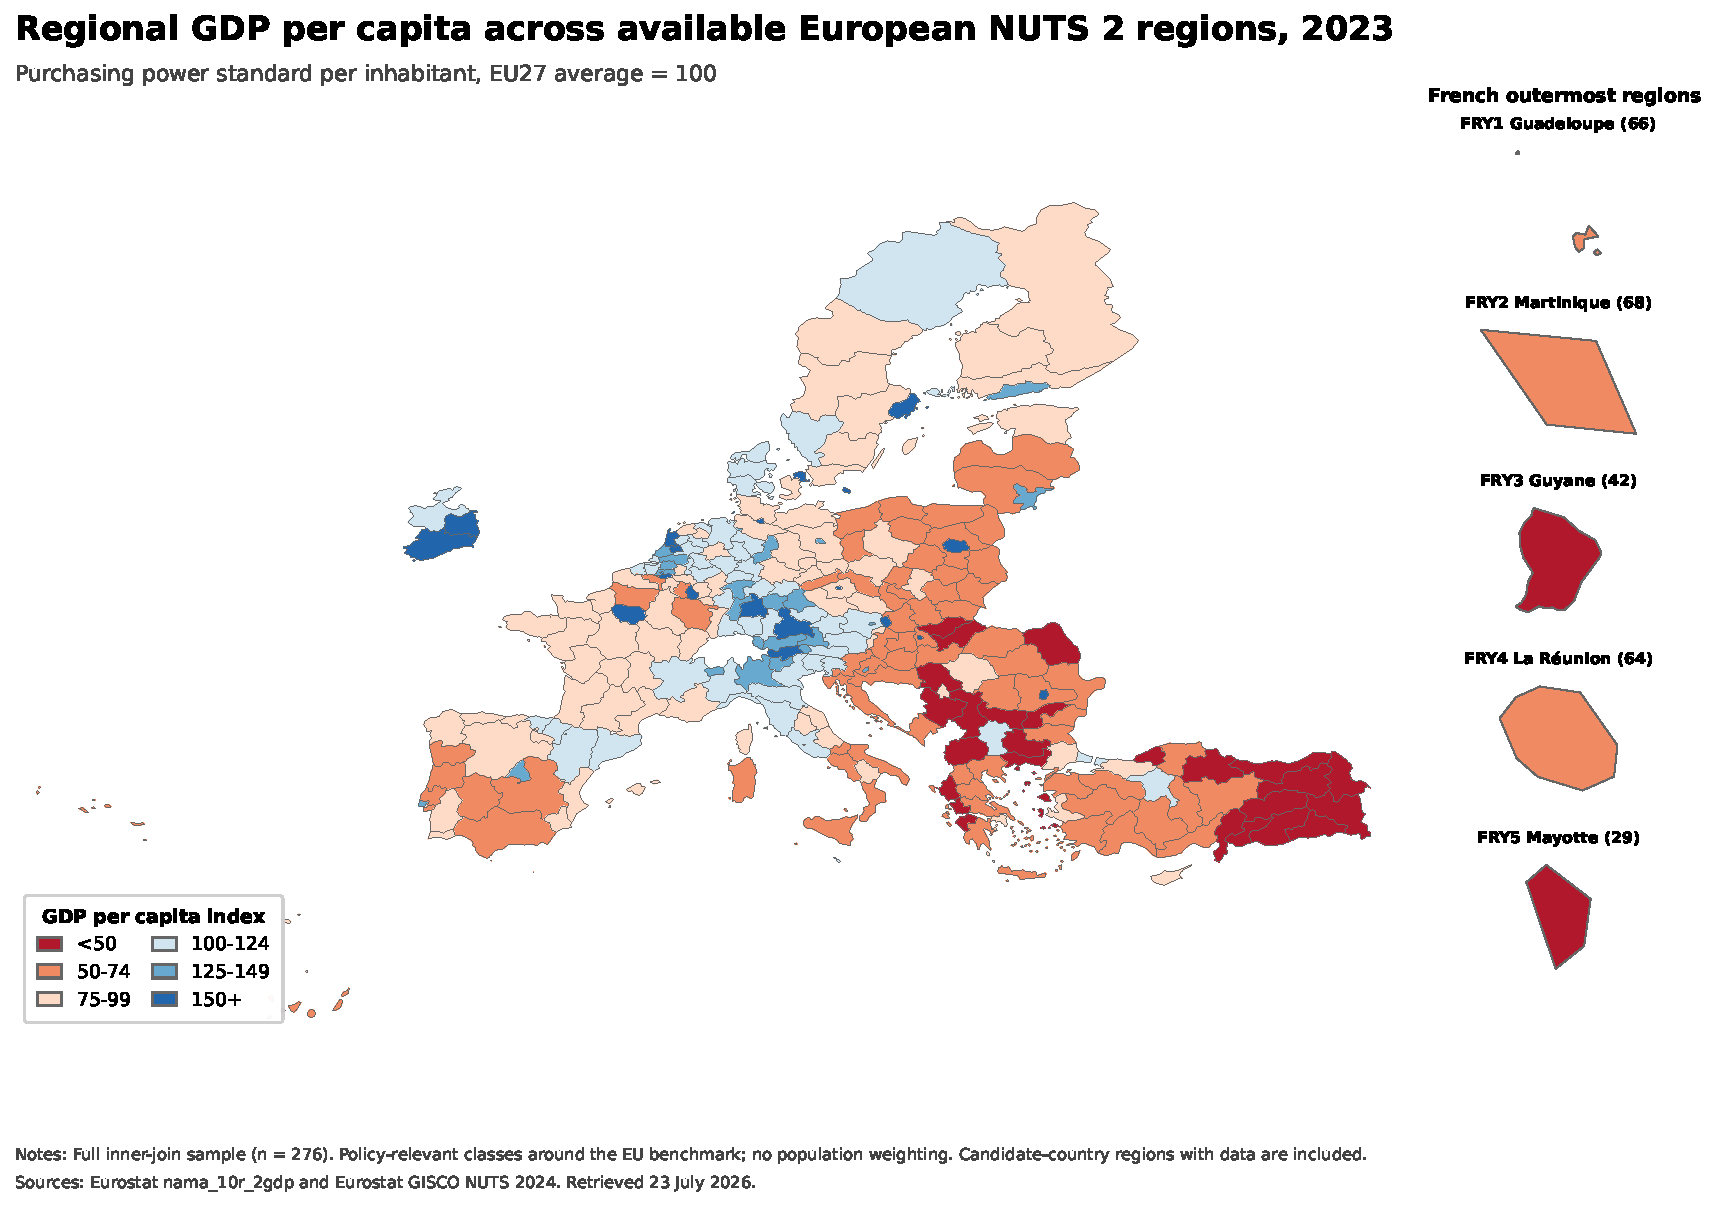
\includegraphics[width=\textwidth]{gdp_per_capita_map.pdf}
\caption{GDP per capita by NUTS 2 region}
\label{fig:gdpmap}
\end{figure}

\subsection{Global spatial association}

\begin{table}[H]
\centering
\caption{Global Moran results and sensitivity checks}
\label{tab:moran}
\resizebox{\textwidth}{!}{\begin{tabular}{lrrrr}
\toprule
Specification & $n$ & Moran's $I$ & $E[I]$ & Permutation $p$ \\
\midrule
Primary: log, queen & 255 & 0.600 & -0.004 & 0.00001 \\
Raw index, queen & 255 & 0.460 & -0.004 & 0.00001 \\
Rank-normalized, queen & 255 & 0.587 & -0.004 & 0.00001 \\
Log, rook & 255 & 0.599 & -0.004 & 0.00001 \\
EU27 only: log, queen & 223 & 0.503 & -0.005 & 0.00001 \\
Largest component: log, queen & 238 & 0.600 & -0.004 & 0.00001 \\
Largest component: log, symmetric 5-NN & 238 & 0.552 & -0.004 & 0.00001 \\
\bottomrule
\end{tabular}
}
\begin{minipage}{0.96\textwidth}
\vspace{0.4em}\footnotesize
\textit{Notes:} All specifications use \Permutations{} one-sided random-label
permutations with fixed, recorded seeds. Queen and rook samples omit only
zero-neighbor regions. The nearest-neighbor graph is symmetric and restricted
to the largest component; its centroids use EPSG:3035.
\end{minipage}
\end{table}

The primary Moran estimate is \MoranI{}, far above its random-label expectation
of approximately $-0.004$, with the minimum attainable permutation
$p$-value of \MoranP{} (Table~\ref{tab:moran}). A region with high log GDP per
capita therefore tends to have high-valued polygon neighbors, and the same is
true for low values. Moran's $I$ is a measure of arrangement, not the magnitude
of inequality summarized by the Gini or Theil index.

The conclusion is insensitive to reasonable choices. The raw-index estimate is
\MoranRawI{}, showing that the result is not created by logs. Rook contiguity
gives \MoranRookI{}. Restricting the sample to EU27 regions reduces the estimate
to \MoranEUI{} but leaves a large positive pattern. Results for the largest
component and its projected nearest-neighbor graph are likewise strongly
positive. Figure~\ref{fig:scatter} displays the global relationship.

\begin{figure}[H]
\centering
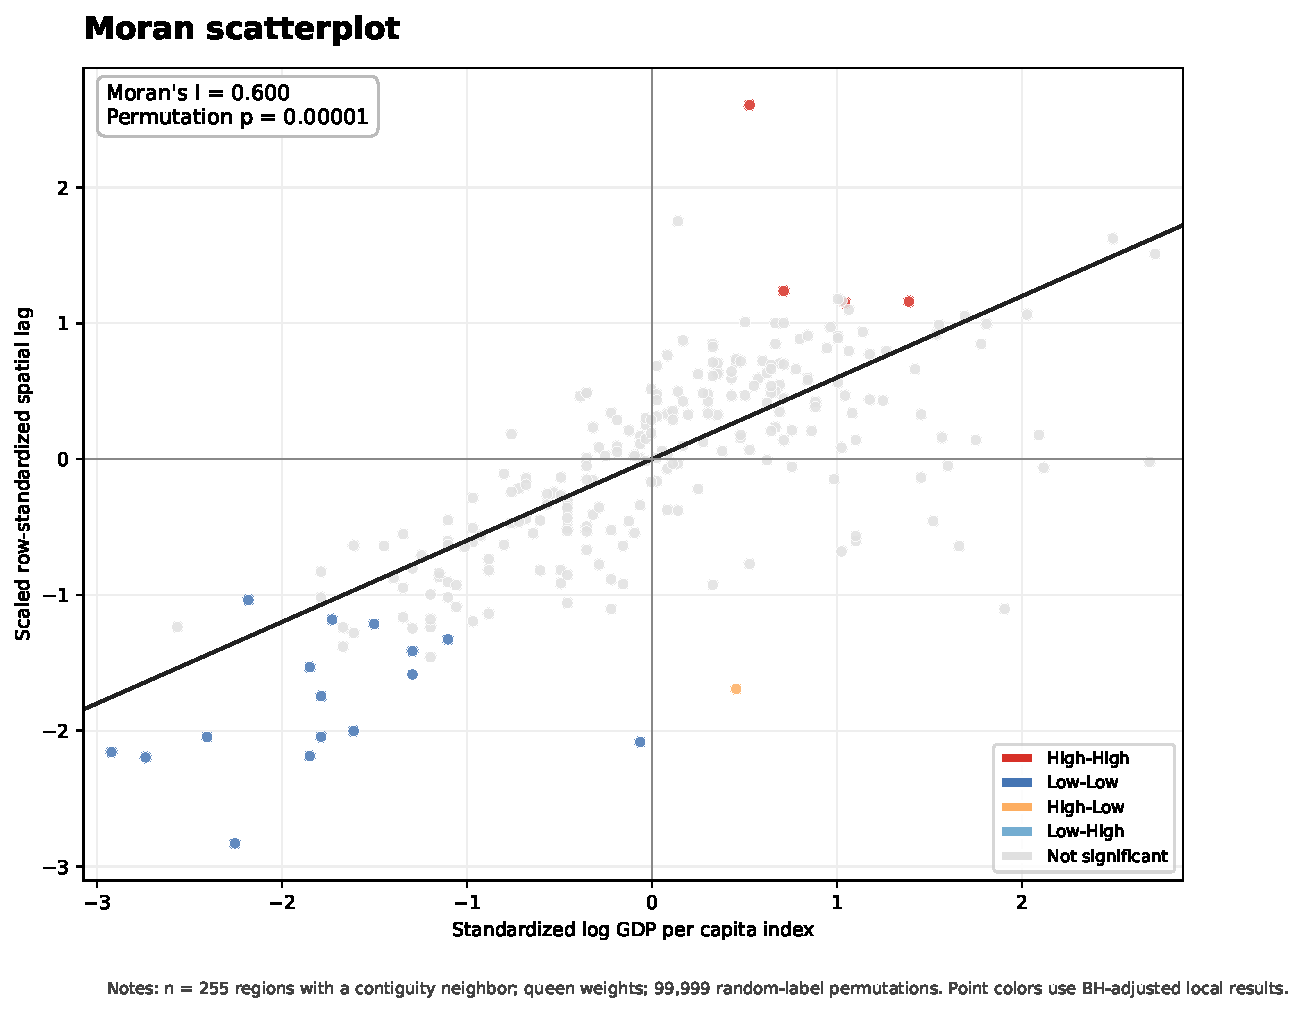
\includegraphics[width=0.82\textwidth]{moran_scatterplot.pdf}
\caption{Moran scatterplot for the primary specification}
\label{fig:scatter}
\end{figure}

\subsection{Local clusters and spatial outliers}

\begin{table}[H]
\centering
\caption{Local Moran classifications after multiplicity adjustment}
\label{tab:lisa}
\begin{tabular}{lrr}
\toprule
Category & BH $q\leq0.05$ & Holm \\
\midrule
High-High & 4 & 1 \\
Low-Low & 16 & 7 \\
High-Low & 1 & 1 \\
Low-High & 0 & 0 \\
Not significant & 234 & 246 \\
No contiguity neighbor & 21 & 21 \\
\bottomrule
\end{tabular}

\begin{minipage}{0.72\textwidth}
\vspace{0.4em}\footnotesize
\textit{Notes:} Counts cover the full joined sample. The \QueenIsolates{}
zero-neighbor regions are shown separately and are not tested.
The first result column applies Benjamini-Hochberg adjustment at $q=0.05$;
the second applies the dependence-robust Holm family-wise-error adjustment at
0.05.
\end{minipage}
\end{table}

Local inference is intentionally more conservative than the global test.
Benjamini-Hochberg retains \LISAFDRTotal{} regions: \LISAHH{} HH,
\LISALL{} LL, \LISAHL{} HL, and \LISALH{} LH
(Table~\ref{tab:lisa}). The HH cores are Salzburg and Tirol in Austria,
Schwaben in Germany, and Northern and Western Ireland. The LL cores lie mainly
across eastern and southeastern Türkiye, with additional regions in Serbia,
Bulgaria, and northern Greece. Yugozapaden, which contains Sofia, is the single
HL spatial outlier: its index is high relative to the analysis center while
its contiguous neighbors have a low spatial lag. These are cluster cores under
the chosen graph, not complete economic ``clubs.''

Only \LISAHolmTotal{} local results survive Holm adjustment. The contrast
between pervasive global association and a short list of local survivors is
not contradictory: global Moran aggregates weakly aligned edges across the
entire graph, whereas each local test faces a stringent multiplicity burden.
Figure~\ref{fig:lisamap} reports the BH-adjusted categories and explicitly
marks regions without a contiguity neighbor.

\begin{figure}[H]
\centering
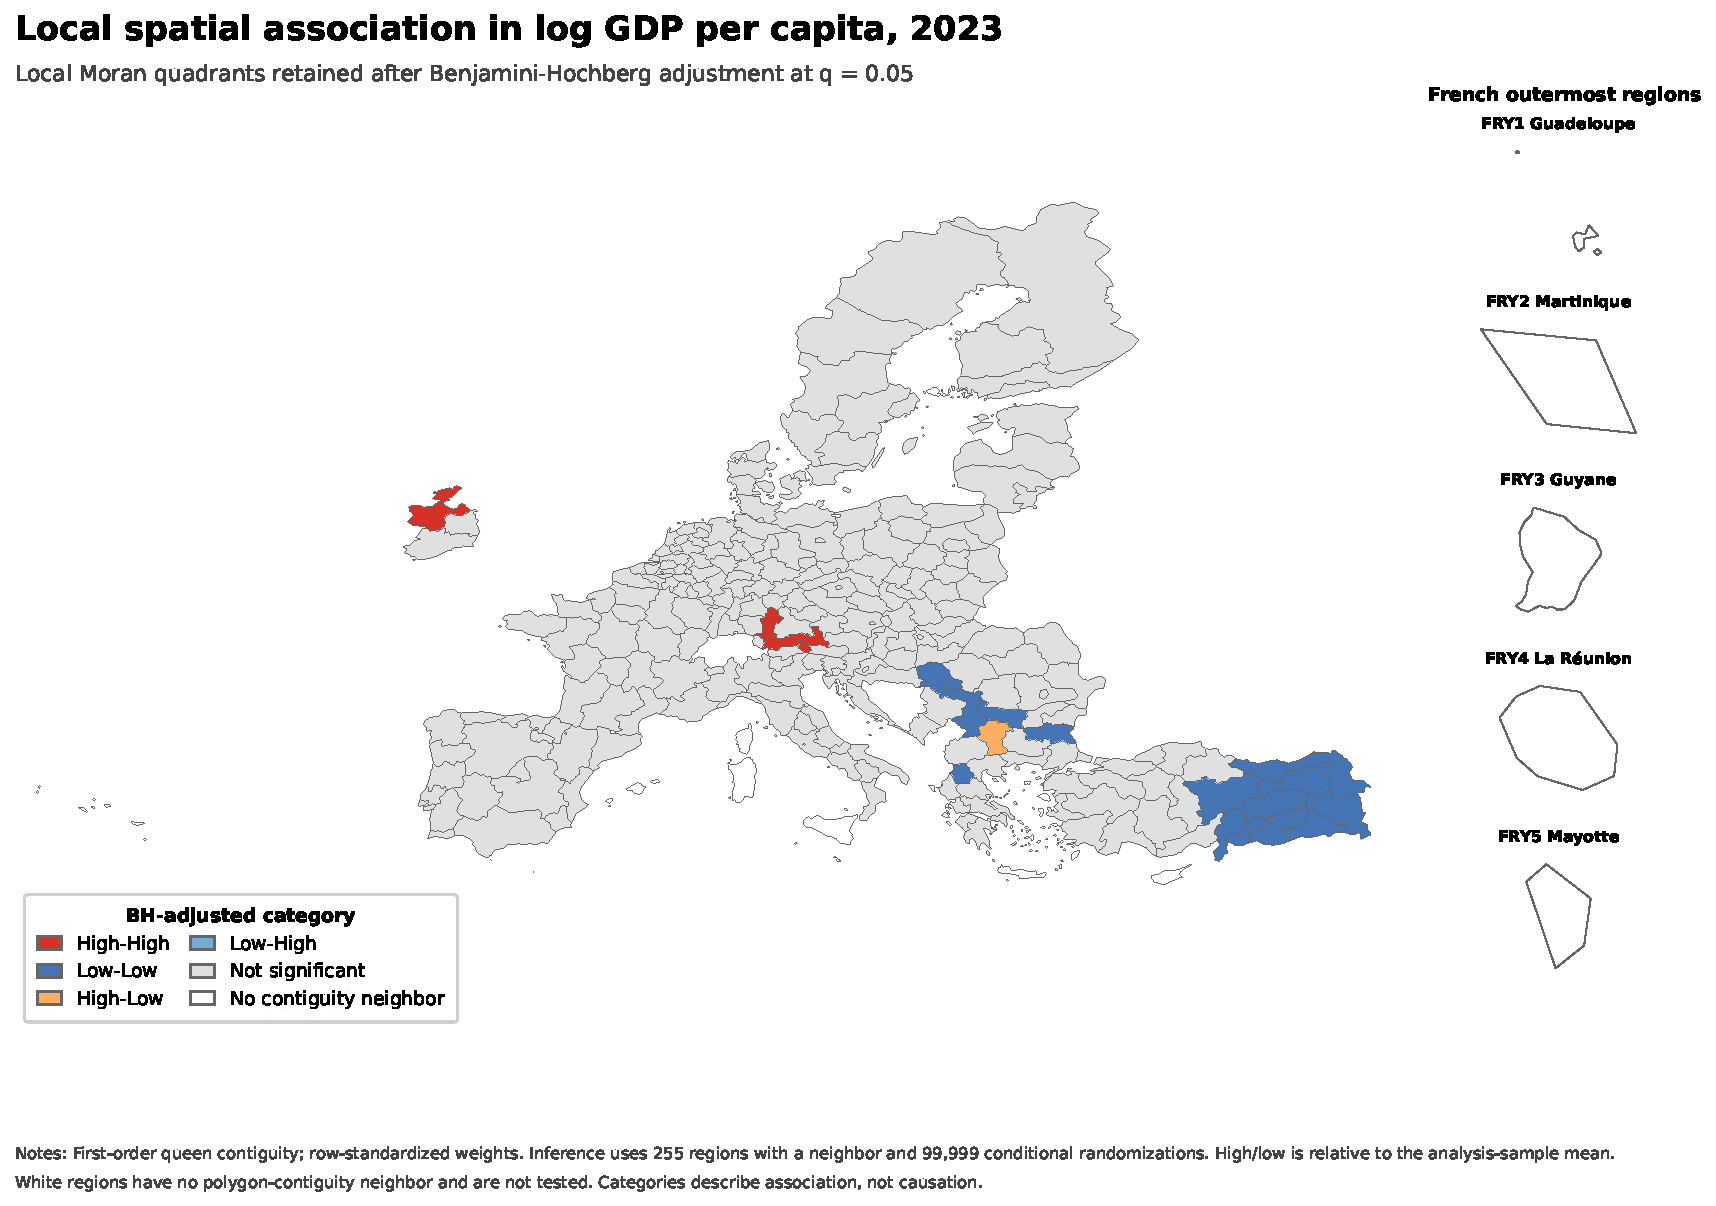
\includegraphics[width=\textwidth]{local_moran_cluster_map.pdf}
\caption{Benjamini-Hochberg-adjusted local Moran clusters}
\label{fig:lisamap}
\end{figure}

\section{Limitations}

Several limitations bound the interpretation.

\begin{itemize}
  \item \textbf{Cross-section.} One year cannot establish beta convergence,
  sigma convergence, persistence, or a change in inequality.
  \item \textbf{No causal design.} Spatial association is compatible with many
  mechanisms, including market access, national institutions, industrial
  structure, sorting, common shocks, and shared history. Moran's $I$ does not
  identify spillovers or policy effects.
  \item \textbf{Production versus welfare.} Regional GDP is workplace
  production, not household living standards. Commuting and multinational
  profit attribution can produce exceptional capital or corporate regions
  \citep{eurostat2025regionalgdp}. National rather than regional price
  converters may conceal subnational cost-of-living differences.
  \item \textbf{Coverage and revisions.} The available-data sample omits EFTA,
  the United Kingdom, and several Balkan regions. \NProvisional{} observations
  are provisional and \NEstimated{} is estimated. Eurostat serves the latest
  vintage, so future downloads may differ from the hashed snapshot.
  \item \textbf{Zoning and geometry.} Results are conditional on NUTS 2024
  boundaries and 1:20 million generalized polygons. The modifiable areal unit
  problem and boundary generalization can affect both dispersion and
  adjacency. Twenty-one island, outermost, or otherwise geographically
  disconnected regions cannot enter the primary contiguity statistic.
  \item \textbf{Permutation null.} Random labeling answers whether this graph
  is more spatially organized than arbitrary reassignment. It is not a
  superpopulation sampling model and does not account for measurement error.
  \item \textbf{Multiple testing.} Local Moran tests overlap spatially.
  Therefore, BH-adjusted values are reported at nominal $q=0.05$ without
  claiming guaranteed false-discovery-rate control. Holm provides a
  dependence-robust family-wise-error check.
\end{itemize}

\section{Conclusion}

Regional GDP per capita in the available Eurostat NUTS 2 cross-section is both
unequal and spatially organized. The region-equal Gini coefficient of
\GiniGDP{} and 90-to-10 ratio of \PninetyTen{} summarize a wide distribution;
country means explain just over half of log variation, leaving substantial
within-country heterogeneity. Global Moran's $I$ of \MoranI{} shows that this
distribution is not randomly arranged over contiguous regions. The positive
association persists in every prespecified sensitivity check.

Local evidence locates a small set of high-high cores in central Europe and
Ireland and a larger low-low concentration in the southeast, but only
\LISAFDRTotal{} regions are retained after BH adjustment, and only
\LISAHolmTotal{} survive Holm adjustment. The appropriate conclusion is
descriptive: Europe's regional production geography in 2023 exhibited strong
spatial clustering. Explaining that geography requires longitudinal data and
a research design capable of separating agglomeration, institutions,
composition, and policy.

\section*{Data and code availability}

All code, raw snapshots, hashes, metadata, anti-joins, processed data, spatial
weights, tables, figures, and build instructions are stored with this paper.
The analysis uses only official Eurostat and GISCO inputs. Re-running the
download script may retrieve a revised vintage; reproducing the reported
numbers requires the archived raw files and recorded checksums.

\clearpage
\bibliographystyle{plainnat}
\bibliography{../references/references}

\end{document}
